\documentclass[8pt]{beamer}

\usetheme[progressbar=frametitle]{metropolis}
\usepackage{appendixnumberbeamer}
\usepackage[style=authoryear, backend=bibtex8, natbib=true, maxcitenames=2]{biblatex}

\usepackage[utf8]{inputenc} % utf8x  defines more symbols, but may cause compatible problems
\usepackage{lmodern,textcomp} % Latin Modern fonts, contains €

\usepackage{graphicx}
\usepackage{import}

\usepackage{booktabs}
\usepackage[scale=2]{ccicons}

\usepackage{pgfplots}
\usepgfplotslibrary{dateplot}

\usepackage{xspace}
\newcommand{\themename}{\textbf{\textsc{metropolis}}\xspace}

\usepackage{amsmath}
\usepackage{bm} % bold symbol in math mode

\usepackage{ulem} % use the "sout" tag to "strikethrough" text
\usepackage[super,negative]{nth} % allows writing 1st, 2nd, 3rd with superscript

\usepackage{tikz}
  \newcommand{\ditto}{
      \tikz{
          \draw [line width=0.12ex] (-0.2ex,0) -- +(0,0.8ex)
              (0.2ex,0) -- +(0,0.8ex);
          \draw [line width=0.08ex] (-0.6ex,0.4ex) -- +(-1.0em,0)
              (0.6ex,0.4ex) -- +(1.0em,0);
      }
  }

% Select what to do with command \comment:
   \newcommand{\comment}[1]{}  %comment not showed
  % \newcommand{\comment}[1]{\par {\bfseries \color{blue} #1 \par}} %comment showed

% Select what to do with todonotes: i.e. \todo{}, \todo[inline]{}
  % \usepackage[disable]{todonotes} % notes not showed
  \usepackage[draft]{todonotes}   % notes showed

  %\numberwithin{equation}{section}

\addbibresource{bib_corruption}


\titlegraphic{\hfill
\includegraphics[width= \textwidth]{logo}}
\title{"The value of local political connections in a low-corruption environment"}
\subtitle{by Mario Daniel Amore \& Morten Bennedsen (2013)}
\date{\today}
\author{Thor Donsby Noe}
\institute{Regulation, Privatization \& Institutions \\
          w. Germà Bel}
%\institute{Department of Economics, University of Copenhagen}

    % \definecolor{BlueTOL}{HTML}{222255}
    \definecolor{BrownTOL}{HTML}{666633}
    \definecolor{GreenTOL}{HTML}{225522}
    % \setbeamercolor{normal text}{fg=BlueTOL,bg=white}
    \setbeamercolor{alerted text}{fg=BrownTOL}
    \setbeamercolor{example text}{fg=GreenTOL}

    \setbeamercolor{block title alerted}{use=alerted text,
        fg=alerted text.fg,
        bg=}
    \setbeamercolor{block body alerted}{use={block title alerted, alerted text},
        fg=alerted text.fg,
        bg=}
    \setbeamercolor{block title example}{use=example text,
        fg=example text.fg,
        bg=}
    \setbeamercolor{block body example}{use={block title example, example text},
        fg=example text.fg,
        bg=}

    \setbeamercolor{block title alerted}{use=alerted text,
        fg=alerted text.fg,
        bg=alerted text.bg!80!alerted text.fg}
    \setbeamercolor{block body alerted}{use={block title alerted, alerted text},
        fg=alerted text.fg,
        bg=block title alerted.bg!50!alerted text.bg}
    \setbeamercolor{block title example}{use=example text,
        fg=example text.fg,
        bg=example text.bg!80!example text.fg}
    \setbeamercolor{block body example}{use={block title example, example text},
        fg=example text.fg,
        bg=block title example.bg!50!example text.bg}


\begin{document}
\setbeamercolor{background canvas}{bg=white}
\maketitle


% ------------------------------------------------------------------------------
% ------ FRAME -----------------------------------------------------------------
% ------------------------------------------------------------------------------
\begin{frame}{Outline}
  \tableofcontents
\end{frame}


\section{Motivation}


\begin{frame}{Previous work}
  \citet{faccio2006politically} finds national political connections with publicly-traded firms in 35 of 47 countries.
  \begin{itemize}
    \item In high-corruption countries, political connections generate a significant abnormal return.
  \end{itemize}
  Several studies on the value of political connections
  \begin{itemize}
    \item In corrupt countries
    \item For powerful natoinal politicians
    \item In time of severe financial crisis
  \end{itemize}
\end{frame}


\begin{frame}{\nth{1} New contribution}
  The value of family connections in one of the least corrupt countries in the World
  \begin{itemize}
    \item Denmark scored 9.3-9.5 in the Corruption Perception Index through 2001-2011
    \item By 2017: A single \nth{4} place as lowest placement since index started in 1995
  \end{itemize}
  E.g. the 2007 CPI placements:
  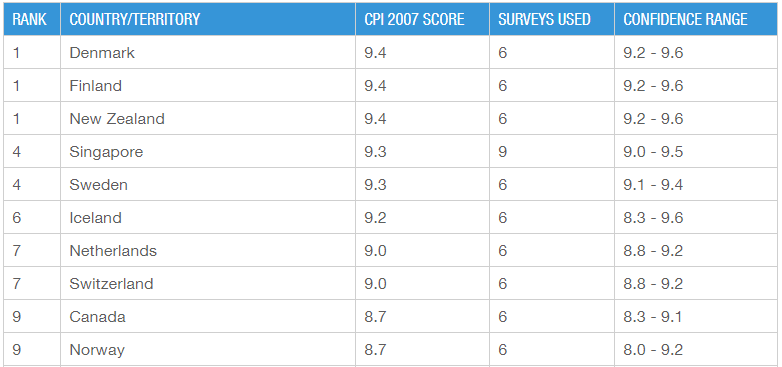
\includegraphics[width= \textwidth]{CPI.PNG}
\end{frame}


\begin{frame}{\nth{2} New contribution}
  The 2005 administrative reform $\rightarrow$ a novel identification strategy
  \begin{itemize}
      \item Differences in differences: 238 municipalities merged into 65
      \item Counterfactuals: 33 municipalities were left unchanged
  \end{itemize}
\end{frame}


\section{Background and data}


\begin{frame}{The 2005 administrative reform}
  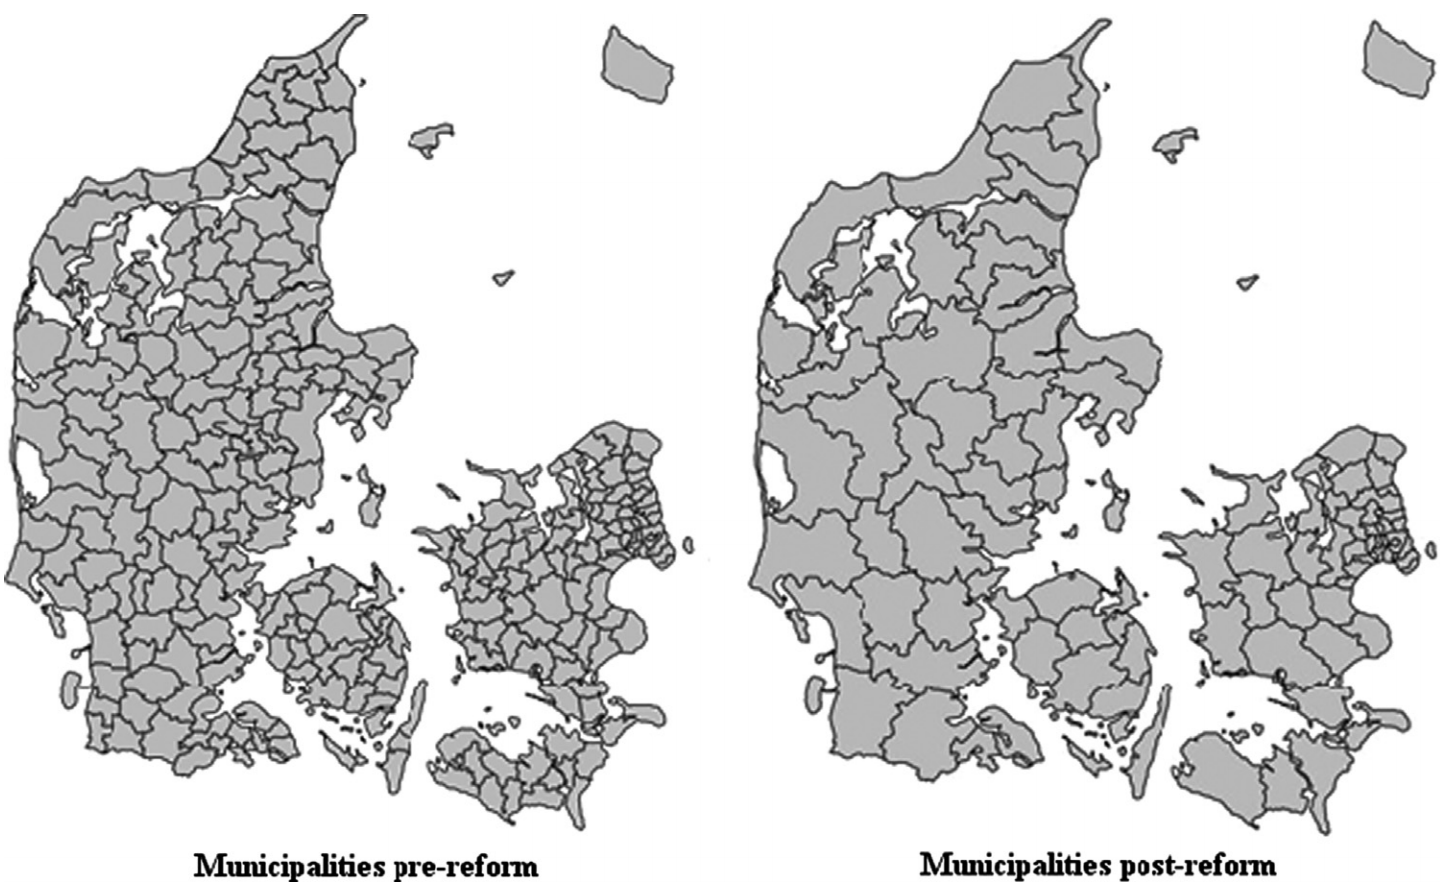
\includegraphics[width= \textwidth]{municipalities.PNG}
\end{frame}


\begin{frame}{The 2005 administrative reform}
  \begin{itemize}
    \item The municipal level accounts for $\sim$48\% of public expenditures.
  \end{itemize}
  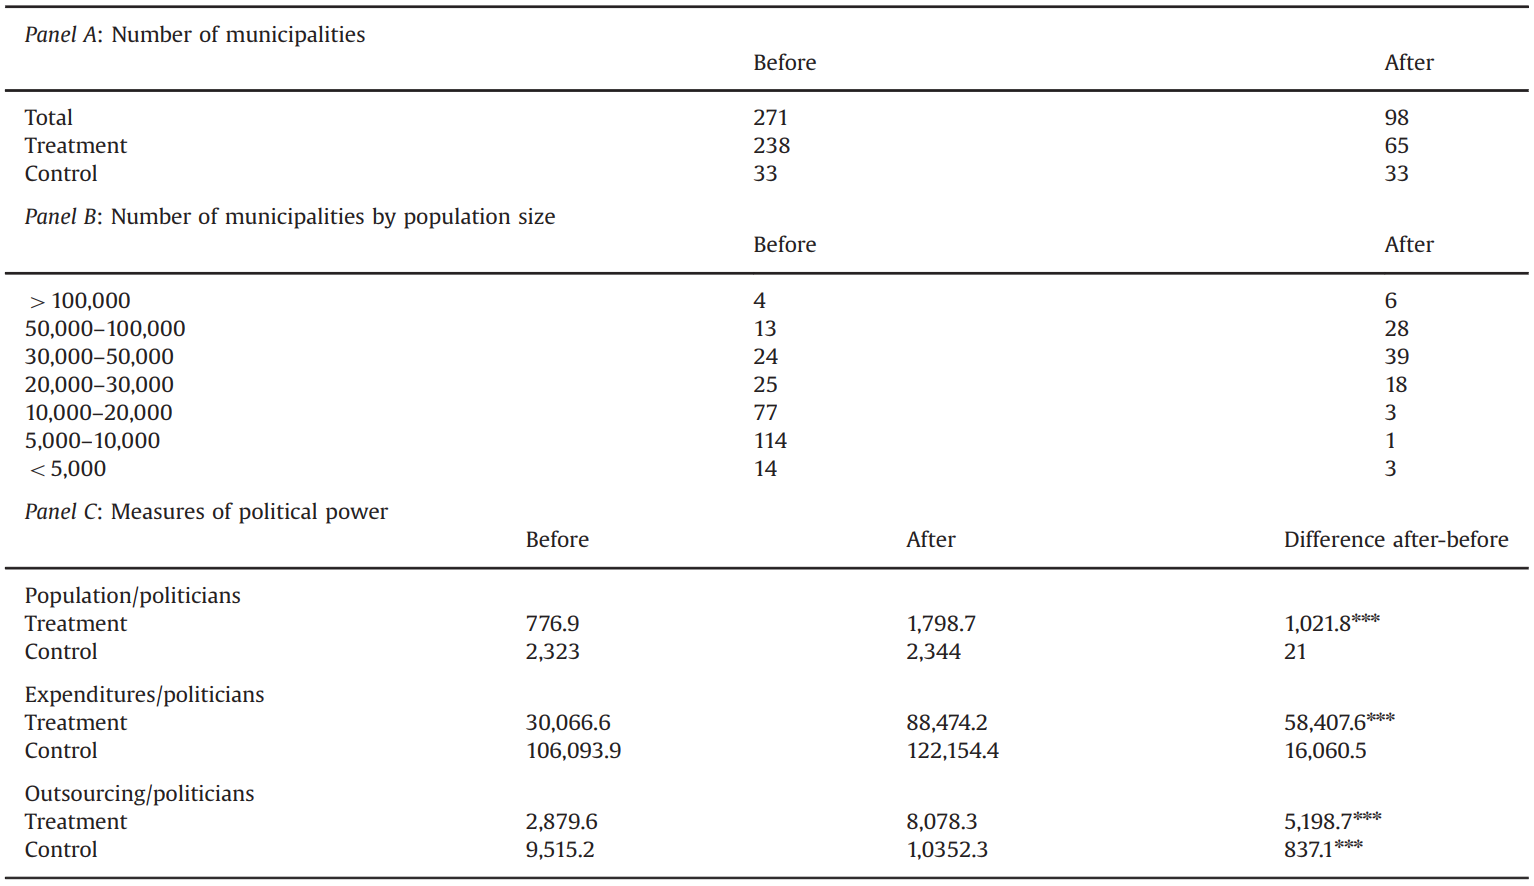
\includegraphics[width= \textwidth]{table1.PNG}
\end{frame}


\begin{frame}{Data}
  Accounting and management data, 2002-2008
  \begin{itemize}
    \item All firms with non-negative book value of total assets.
    \item Profitability (operating and net income).
    \item Annual balance sheets are mandatory and approwed by external accountants.
    \item Obtain personal ID numbers of all managers and board members.
  \end{itemize}
  Electoral data for 2001, 2005, and 2009 local elections
  \begin{itemize}
    \item Electoral data on ID, party affiliation, votes and electoral success/failure
  \end{itemize}
  Family networks and political connections, elections
  \begin{itemize}
    \item Create family trees from merging administrative data
    \item Consider family relations: parent, child, sibling, current/former spouse(s).
  \end{itemize}
\end{frame}


\section{Empirical strategy}


\begin{frame}{Differences-in-differences}
  "How the increase in political power due to the enlargement of local governments increased the profitability of firms connected with local politicians before and after the reform" \citep{amore2013value}
  \begin{itemize}
    \item Premise: Merging of municipalities $\rightarrow$ positive shock to politicians' power.
    \begin{itemize}
      \item Merging more than doubled population/politicans and also tripled expenditures/politicians and outsourcing/politicians.
    \end{itemize}
    \item Counterfactuals: Similarly connected firms in unchanged municipalities.
  \end{itemize}
  Potential endogeneity in other studies:
  \begin{itemize}
    \item Connections to \textit{well-performing} firms can decide election outcomes.
    \item Thus, unnconnected firms or firms connected with unelected candidates $\rightarrow$ poor counterfactuals
  \end{itemize}
\end{frame}


\section{Results}


\begin{frame}{Operating return on assets (OROA)}
  \textbf{Table 5: Difference-in-difference estimates}\\
  Differences between average for 2001-2004 and 2006-2008 for firms connected with reelected politicians. Treatment = merging municipality. Controls: Regional dummies. Depending on specification: lagged log(total assets), lagged industry-ajusted OROA.
  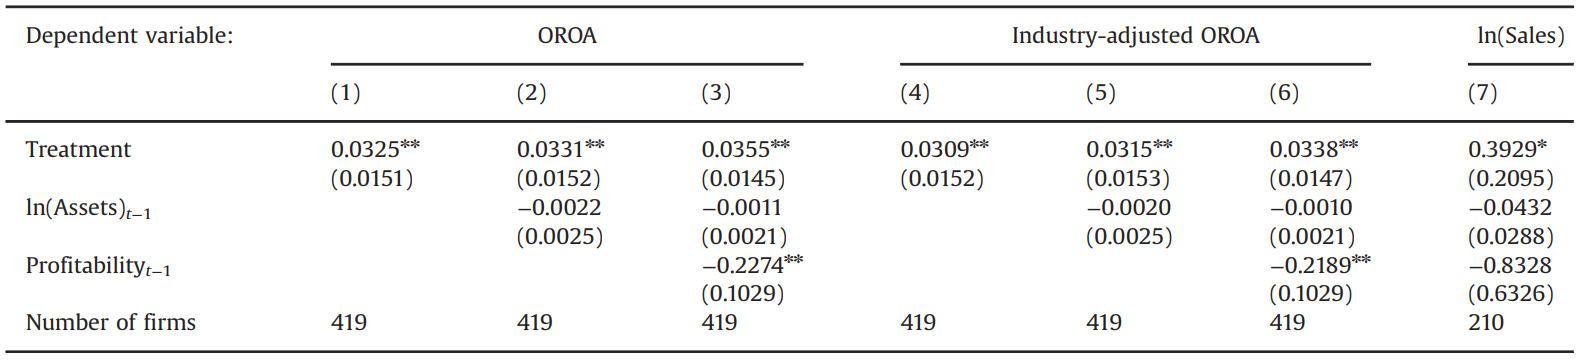
\includegraphics[width= \textwidth]{OROA.PNG}
\end{frame}


\begin{frame}{Sales and public demand}
  \textbf{Table 6: Difference-in-difference estimates}
  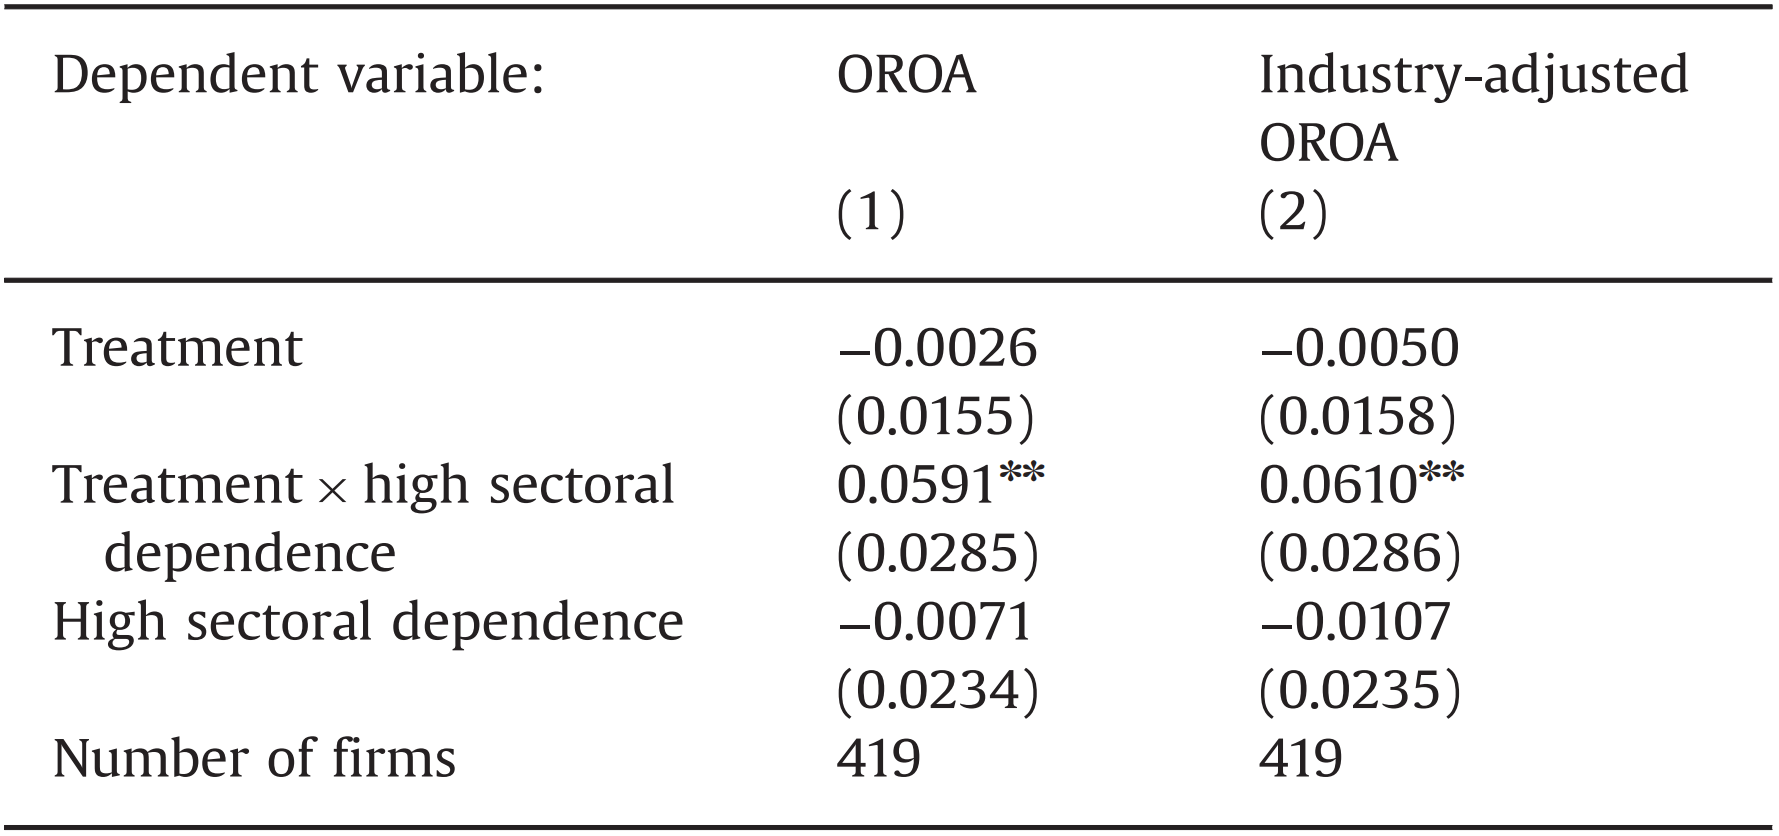
\includegraphics[width= \textwidth]{dependence.PNG}
\end{frame}


\begin{frame}{Main results}
  Profitability more than doubled from treatment
  \begin{itemize}
    \item Difference in OROA is 3.25 pct.-points higher in treated municipalities.
    \item Average profitability was 2.25\% in 2005.
  \end{itemize}
  Elasticity of connected firm performance is
  \begin{itemize}
    \item 1.07 wrt. changes in population per politician
    \item 0.78 wrt. changes in expenditure per politician
    \item 0.81 wrt. changes in outsourcing per politician
  \end{itemize}
  Difference in sales increased by 39\% due to treatment
  \begin{itemize}
    \item Indicate that increased profitability is partly due to higher sales
    \item Only significant at 10\% level, and selection bias as only half of the firms chose to report sales.
  \end{itemize}
  Even more important for firms in sectorws depending on public-demand
  \begin{itemize}
    \item Difference in OROA i 6 pct.-points higher in treated municipalities.
  \end{itemize}
\end{frame}


\begin{frame}{Causal validation}
  \textbf{Falsification, robustness, selection bias, matching and discontinuity}
  \begin{enumerate}
    \item Municipality mergers does not affect the profitability of non-connected firms
    \begin{itemize}
      \item Even though the transition was backed by €160 mio. for merging municipalities only.
    \end{itemize}
    \item No significantly diverging firm-level pre-reform trends between treated and controls
    \item Selection bias due to increased electoral competition in merging municipalities0
    \begin{itemize}
      \item Bias could either be postitive or negative as tougher competition could lead to re-elected politicians being of higher-quality or more reliant on economic support from firms.
      \item Include aggregate party vote and share of politicians older than 65 years in pre-reform municipalities as indicators of toughness of competition.
    \end{itemize}
    \item Using sharp RDD
    \begin{itemize}
      \item Comparing municipalities barely above and below the 20,000 inhabitans threshold.
      \item Thus, results not affected by declining economic or demographic trends.
    \end{itemize}
  \end{enumerate}
\end{frame}


\begin{frame}{Heterogeneous effects}
  Sample split results show
  \begin{enumerate}
    \item Firms benefit more from being connected to stronger politicians.
    \item Firms that benefit from political connections are characterized by
    \begin{itemize}
      \item Being small firms, making little profit pre-reform.
      \item Indicate that rent extraction does not increase overall welfare.
    \end{itemize}
  \end{enumerate}
  Strength and persistence of political institutions matter
  \begin{enumerate}
    \item A smaller effect of treatment in municipalities where electoral competition increased more.
    \item Reduced ability to extract rent for connected firms in municipalities with strong institutions.
    \begin{itemize}
      \item Former 'market towns' (Købstader) which as early as the medieval age received special privileges to self-administrate has persistently improved institutional quality.
    \end{itemize}
  \end{enumerate}
\end{frame}


\section{Conclusion}


\begin{frame}{Main takeaway}
  Family ties with politicians $\rightarrow$ more business with local government.
  \begin{itemize}
    \item Increase in political power highly improves performance of connected firms
    \begin{itemize}
      \normalsize
      \item A 100\% increase in population per politician $\rightarrow$ 107\% increase in firm's profitability.
    \end{itemize}
    \item Greater effect for firms in industries that depend more on public demand.
    \item Tough electoral competition and strong institutions can reduce the effect.
  \end{itemize}
  % Critique: Not similar pre-treatment trends
  % \begin{itemize}
  %   \item In 2005 profitability of connected firms was 3.6\% in treated municipalities and 2.6\% in control municipalities.
  %   \item For firms connected with reelected candidates only, profitability was 2.5\% in treated municipalities and 2.2\% in control municipalities.
  % \end{itemize}
  The public sector is not perceived to be corrupt before nor after the reform.
  \begin{itemize}
    \item Could be because the individual cases are small in economical relevance? As indicated by \citet{pena2018privatization}.
  \end{itemize}
\end{frame}

% \section{References}


\begin{frame}%{References}
  \printbibliography
\end{frame}

%   \begin{figure}[!h]
%   %  \def\svgwidth{0.50\columnwidth}
%   %  \input{tree.pdf_tex}
%     \resizebox{3in}{!}{\input{tree.pdf_tex}}
%   %  \caption{Timeline illustration of event setup}
%   \end{figure}

\end{document}
